\documentclass[11pt]{article}\usepackage[]{graphicx}\usepackage[]{color}
%% maxwidth is the original width if it is less than linewidth
%% otherwise use linewidth (to make sure the graphics do not exceed the margin)
\makeatletter
\def\maxwidth{ %
  \ifdim\Gin@nat@width>\linewidth
    \linewidth
  \else
    \Gin@nat@width
  \fi
}
\makeatother

\definecolor{fgcolor}{rgb}{0.345, 0.345, 0.345}
\newcommand{\hlnum}[1]{\textcolor[rgb]{0.686,0.059,0.569}{#1}}%
\newcommand{\hlstr}[1]{\textcolor[rgb]{0.192,0.494,0.8}{#1}}%
\newcommand{\hlcom}[1]{\textcolor[rgb]{0.678,0.584,0.686}{\textit{#1}}}%
\newcommand{\hlopt}[1]{\textcolor[rgb]{0,0,0}{#1}}%
\newcommand{\hlstd}[1]{\textcolor[rgb]{0.345,0.345,0.345}{#1}}%
\newcommand{\hlkwa}[1]{\textcolor[rgb]{0.161,0.373,0.58}{\textbf{#1}}}%
\newcommand{\hlkwb}[1]{\textcolor[rgb]{0.69,0.353,0.396}{#1}}%
\newcommand{\hlkwc}[1]{\textcolor[rgb]{0.333,0.667,0.333}{#1}}%
\newcommand{\hlkwd}[1]{\textcolor[rgb]{0.737,0.353,0.396}{\textbf{#1}}}%

\usepackage{framed}
\makeatletter
\newenvironment{kframe}{%
 \def\at@end@of@kframe{}%
 \ifinner\ifhmode%
  \def\at@end@of@kframe{\end{minipage}}%
  \begin{minipage}{\columnwidth}%
 \fi\fi%
 \def\FrameCommand##1{\hskip\@totalleftmargin \hskip-\fboxsep
 \colorbox{shadecolor}{##1}\hskip-\fboxsep
     % There is no \\@totalrightmargin, so:
     \hskip-\linewidth \hskip-\@totalleftmargin \hskip\columnwidth}%
 \MakeFramed {\advance\hsize-\width
   \@totalleftmargin\z@ \linewidth\hsize
   \@setminipage}}%
 {\par\unskip\endMakeFramed%
 \at@end@of@kframe}
\makeatother

\definecolor{shadecolor}{rgb}{.97, .97, .97}
\definecolor{messagecolor}{rgb}{0, 0, 0}
\definecolor{warningcolor}{rgb}{1, 0, 1}
\definecolor{errorcolor}{rgb}{1, 0, 0}
\newenvironment{knitrout}{}{} % an empty environment to be redefined in TeX

\usepackage{alltt}
\usepackage{amsmath}
\usepackage{pslatex}
\usepackage{natbib}
\usepackage{setspace}
%\usepackage[sc]{mathpazo}
%\usepackage[T1]{fontenc}
\usepackage[margin=1in,pdftex]{geometry}
\setcounter{secnumdepth}{2}
\setcounter{tocdepth}{2}
\usepackage{url}
\usepackage[unicode=true,pdfusetitle,
 bookmarks=true,bookmarksnumbered=true,bookmarksopen=true,bookmarksopenlevel=2,
 breaklinks=false,pdfborder={0 0 1},backref=false,colorlinks=false]{hyperref}
\hypersetup{pdfstartview={XYZ null null 1}}
\usepackage{breakurl}
%\usepackage[authoryear]{natbib}

\newcommand{\quanteda}{\textsf{quanteda}\ }
\IfFileExists{upquote.sty}{\usepackage{upquote}}{}

\begin{document}
%\SweaveOpts{concordance=TRUE}







\title{Introduction to the Quantitative Analysis of Textual Data Using
  \quanteda\thanks{This research was supported by the European
    Research Council grant ERC-2011-StG 283794-QUANTESS.  Code
    contributors to the project include Alex Herzog, William Lowe, and
    Kohei Watanabe.}}

\author{Kenneth Benoit and Paul Nulty}

\maketitle

\setlength{\parskip}{1ex}
\setlength{\parindent}{0ex}

\section{Introduction: The Rationale for \quanteda}

\quanteda is an R package designed to simplify the process of
quantitative analysis of text from start to finish, making it possible
to turn texts into a structured corpus, conver this corpus into a
quantitative matrix of features extracted from the texts, and to
perform a variety of quanttative analyses on this matrix.  The object
is inference about the data contained in the texts, whether this means
describing characteristics of the texts, inferring quantities of
interests about the texts of their authors, or determining the tone or
topics contained in the texts.  The emphasis of \quanteda is on
\emph{simplicity}: creating a corpus to manage texts and variables
attached to these texts in a straightforward way, and providing
powerful tools to extract features from this corpus that can be
analyzed using quantitative techniques.

The tools for getting texts into a corpus object include: 
\begin{itemize}
\item loading texts from directories of individual files
\item loading texts ``manually'' by inserting them into a corpus using
  helper functions
\item managing text encodings and conversions from source files into
  corpus texts
\item attaching variables to each text that can be used for grouping,
  reorganizing a corpus, or simply recording additional information to
  supplement quantitative analyses with non-textual data
\item recording meta-data about the sources and creation details for
  the corpus.
\end{itemize}

The tools for working with a corpus include:
\begin{itemize}
\item summarizing the corpus in terms of its language units
\item reshaping the corpus into smaller units or more aggregated units
\item adding to or extracting subsets of a corpus
\item resampling texts of the corpus, for example for use in
  non-parametric bootstrapping of the texts \citep[for an example, see][]{lowebenoitPA2013}
  \item Easy extraction and saving, as a new data frame or corpus, key
    words in context (KWIC)
\end{itemize}

For extracting features from a corpus, \quanteda provides the following tools:
\begin{itemize}
\item extraction of word types
\item extraction of word $n$-grams
\item extraction of dictionary entries from user-defined dictionaries
\item feature selection through
  \begin{itemize}
  \item stemming
  \item random selection
  \item document frequency
  \item word frequency
  \item and a variety of options for cleaning word types, such as
    capitalization and rules for handling punctuation.
  \end{itemize}
\end{itemize}

For analyzing the resulting \emph{document-feature} matrix created
when features are abstracted from a corpus, \quanteda provides:
\begin{itemize}
\item scaling models, such as the Poisson scaling model or Wordscores
\item nonparametric visualization, such as correspondence analysis
\item topic models, such as LDA
\item classifiers, such as Naive Bayes or $k$-nearest neighbour
\item sentiment analysis, using dictionaries
\end{itemize}

\quanteda is hardly unique in providing facilities for working with
text -- the excellent \textsf{tm} package already provides many of the
features we have described.  \quanteda is designed to complement those
packages, as well to simplify the implementation of the
text-to-analysis workflow.  \quanteda corpus structures are simpler
objects than in \textsf{tm}, as are the document-feature matrix
objects from \quanteda, compared to the sparse matrix implementation
found in \textsf{tm}.  However, there is no need to choose only one
package, since we provide translator functions from one matrix or
corpus object to the other in \quanteda.

This vignette is designed to introduce you to \quanteda as well as
provide a tutorial overview of its features.

\section{Installing \quanteda}

The code for the \quanteda package currently resides on
\url{http://github/kbenoit/quanteda}.  From an Internet-connected
computer, you can install the package directly using the
\textsf{devtools} package:

\begin{knitrout}
\definecolor{shadecolor}{rgb}{0.969, 0.969, 0.969}\color{fgcolor}\begin{kframe}
\begin{alltt}
\hlkwd{library}\hlstd{(devtools)}
\hlkwa{if} \hlstd{(}\hlopt{!}\hlkwd{require}\hlstd{(quanteda))} \hlkwd{install_github}\hlstd{(}\hlstr{"quanteda"}\hlstd{,} \hlkwc{username} \hlstd{=} \hlstr{"kbenoit"}\hlstd{)}
\end{alltt}


{\ttfamily\noindent\itshape\color{messagecolor}{\#\# Loading required package: quanteda}}\end{kframe}
\end{knitrout}


For other branches, for instance if you wish to install the
\texttt{dev} branch (containing work in progress) rather than the
master, you should instead run

\begin{knitrout}
\definecolor{shadecolor}{rgb}{0.969, 0.969, 0.969}\color{fgcolor}\begin{kframe}
\begin{alltt}
\hlkwd{install_github}\hlstd{(}\hlstr{"quanteda"}\hlstd{,} \hlkwc{username} \hlstd{=} \hlstr{"kbenoit"}\hlstd{,} \hlkwc{ref} \hlstd{=} \hlstr{"dev"}\hlstd{)}
\end{alltt}
\end{kframe}
\end{knitrout}




\section{Creating a corpus}

\subsection{Loading Documents into Quanteda}

\subsubsection{From a directory of files}

A very common source of files for creating a corpus will be a set of
text files found on a local (or remote) directory.  To load in a set
of these files, we will load a corpus from a set of text files using
information on attributes of the text that have been conveniently
stored in the text document's filename (separated by underscores).
For example, for our corpus of Irish budget speeches, the filename
\texttt{2010\_BUDGET\_03\_Joan\_Burton\_LAB.txt} tells us the year of
the speech (2010), the type (``BUDGET''), a serial number (03), the
first and last name of the speaker, and a party label (``LAB'' for
Labour).

To load this into a corpus object, we will use the
\texttt{corpusFromFilenames} function, supplying a vector of attribute
labels that correspond with the elements of the filename.

\begin{knitrout}
\definecolor{shadecolor}{rgb}{0.969, 0.969, 0.969}\color{fgcolor}\begin{kframe}
\begin{alltt}
\hlkwd{library}\hlstd{(quanteda)}
\hlstd{textfile} \hlkwb{<-} \hlstr{"https://github.com/kbenoit/quanteda/blob/dev/texts/irishbudgets2010.zip?raw=true"}
\hlkwd{download.file}\hlstd{(textfile,} \hlkwd{basename}\hlstd{(textfile),} \hlkwc{method} \hlstd{=} \hlstr{"curl"}\hlstd{,} \hlkwc{extra} \hlstd{=} \hlstr{"-L"}\hlstd{)}  \hlcom{# download this zipped archive of texts}
\hlkwd{unzip}\hlstd{(}\hlkwd{basename}\hlstd{(textfile))}  \hlcom{# unzip the file}
\hlstd{attNames} \hlkwb{<-} \hlkwd{c}\hlstd{(}\hlstr{"year"}\hlstd{,} \hlstr{"debate"}\hlstd{,} \hlstr{"number"}\hlstd{,} \hlstr{"firstname"}\hlstd{,} \hlstr{"surname"}\hlstd{,} \hlstr{"party"}\hlstd{)}
\hlstd{ieBudgets2010} \hlkwb{<-} \hlkwd{corpusFromFilenames}\hlstd{(}\hlstr{"budget_2010"}\hlstd{,} \hlkwd{c}\hlstd{(}\hlstr{"year"}\hlstd{,} \hlstr{"debate"}\hlstd{,} \hlstr{"no"}\hlstd{,} \hlstr{"fname"}\hlstd{,}
    \hlstr{"speaker"}\hlstd{,} \hlstr{"party"}\hlstd{),} \hlkwc{sep} \hlstd{=} \hlstr{"_"}\hlstd{)}
\end{alltt}
\end{kframe}
\end{knitrout}


This creates a new quanteda corpus object where each text has been associated values for its attribute types extracted from the filename:

\begin{knitrout}
\definecolor{shadecolor}{rgb}{0.969, 0.969, 0.969}\color{fgcolor}\begin{kframe}
\begin{alltt}
\hlkwd{summary}\hlstd{(ieBudgets2010)}
\end{alltt}
\begin{verbatim}
## Corpus object contains 14 texts.
## 
##                                      Texts Types Tokens Sentences year debate
##        2010_BUDGET_01_Brian_Lenihan_FF.txt  1655   7799       390 2010 BUDGET
##       2010_BUDGET_02_Richard_Bruton_FG.txt   956   4058       222 2010 BUDGET
##         2010_BUDGET_03_Joan_Burton_LAB.txt  1485   5770       329 2010 BUDGET
##        2010_BUDGET_04_Arthur_Morgan_SF.txt  1463   6481       349 2010 BUDGET
##          2010_BUDGET_05_Brian_Cowen_FF.txt  1473   5880       262 2010 BUDGET
##           2010_BUDGET_06_Enda_Kenny_FG.txt  1066   3875       161 2010 BUDGET
##      2010_BUDGET_07_Kieran_ODonnell_FG.txt   614   2066       141 2010 BUDGET
##       2010_BUDGET_08_Eamon_Gilmore_LAB.txt  1098   3800       208 2010 BUDGET
##     2010_BUDGET_09_Michael_Higgins_LAB.txt   447   1136        49 2010 BUDGET
##        2010_BUDGET_10_Ruairi_Quinn_LAB.txt   418   1177        60 2010 BUDGET
##      2010_BUDGET_11_John_Gormley_Green.txt   363    929        49 2010 BUDGET
##        2010_BUDGET_12_Eamon_Ryan_Green.txt   482   1513        90 2010 BUDGET
##      2010_BUDGET_13_Ciaran_Cuffe_Green.txt   423   1143        48 2010 BUDGET
##  2010_BUDGET_14_Caoimhghin_OCaolain_SF.txt  1055   3654       194 2010 BUDGET
##  no      fname  speaker party
##  14 Caoimhghin OCaolain    SF
##  13     Ciaran    Cuffe Green
##  12      Eamon     Ryan Green
##  11       John  Gormley Green
##  10     Ruairi    Quinn   LAB
##  09    Michael  Higgins   LAB
##  08      Eamon  Gilmore   LAB
##  07     Kieran ODonnell    FG
##  06       Enda    Kenny    FG
##  05      Brian    Cowen    FF
##  04     Arthur   Morgan    SF
##  03       Joan   Burton   LAB
##  02    Richard   Bruton    FG
##  01      Brian  Lenihan    FF
## 
## Source:  /home/paul/Dropbox/code/quanteda/vignettes/* on x86_64 by paul.
## Created: Tue Jun  3 18:09:56 2014.
## Notes:   NA.
\end{verbatim}
\end{kframe}
\end{knitrout}


\subsubsection{From a vector of texts}


\subsection{Adding Information to a corpus}

\subsubsection{Adding new texts}

\subsubsection{Adding new text attributes}


\subsection{Translating a \quanteda corpus into other formats}

\subsubsection{Importing from QDAMiner}

\subsubsection{Importing to and exporting from \textsf{tm}}


\section{Manipulating a corpus}


\section{Extracting Features}


\section{Analyzing a document-feature matrix}





% \singlespacing
\bibliographystyle{apsr}
\bibliography{../../bibliographies/QUANTESS}

\end{document}


In order to perform statistical analysis such as document scaling, we must extract a matrix containing the frequency of each word type from in document. In quanteda, we use the dfm function to produce such a matrix. \footnote{dfm stands for document-feature matrix --- we say `feature' instead of word, as it is sometimes useful to represent documents by features other than their word frequency.}

\begin{knitrout}
\definecolor{shadecolor}{rgb}{0.969, 0.969, 0.969}\color{fgcolor}\begin{kframe}
\begin{alltt}
\hlstd{docMat} \hlkwb{<-} \hlkwd{dfm}\hlstd{(ieBudgets2010)}
\end{alltt}
\begin{verbatim}
## Creating dfm: ... done.
\end{verbatim}
\begin{alltt}
\hlstd{docMat[}\hlnum{1}\hlopt{:}\hlnum{5}\hlstd{,} \hlnum{1}\hlopt{:}\hlnum{5}\hlstd{]}
\end{alltt}
\begin{verbatim}
##                                       words
## docs                                    €  —   a abandoned abandoning
##   2010_BUDGET_01_Brian_Lenihan_FF.txt  75  4 143         0          0
##   2010_BUDGET_02_Richard_Bruton_FG.txt 18  5  82         1          0
##   2010_BUDGET_03_Joan_Burton_LAB.txt   48 11 129         1          0
##   2010_BUDGET_04_Arthur_Morgan_SF.txt  42  7 115         0          1
##   2010_BUDGET_05_Brian_Cowen_FF.txt    38  7 122         0          0
\end{verbatim}
\end{kframe}
\end{knitrout}


We can now score and plot the documents using a statistical scaling technique, for example correspondence analysis.

\begin{knitrout}
\definecolor{shadecolor}{rgb}{0.969, 0.969, 0.969}\color{fgcolor}\begin{kframe}
\begin{alltt}
\hlkwd{library}\hlstd{(ca)}
\hlstd{model} \hlkwb{<-} \hlkwd{ca}\hlstd{(}\hlkwd{t}\hlstd{(docMat),} \hlkwc{nd} \hlstd{=} \hlnum{1}\hlstd{)}
\hlkwd{dotchart}\hlstd{(model}\hlopt{$}\hlstd{colcoord[}\hlkwd{order}\hlstd{(model}\hlopt{$}\hlstd{colcoord[,} \hlnum{1}\hlstd{]),} \hlnum{1}\hlstd{],} \hlkwc{labels} \hlstd{= model}\hlopt{$}\hlstd{colnames[}\hlkwd{order}\hlstd{(model}\hlopt{$}\hlstd{colcoord[,}
    \hlnum{1}\hlstd{])])}
\end{alltt}
\end{kframe}

{\centering 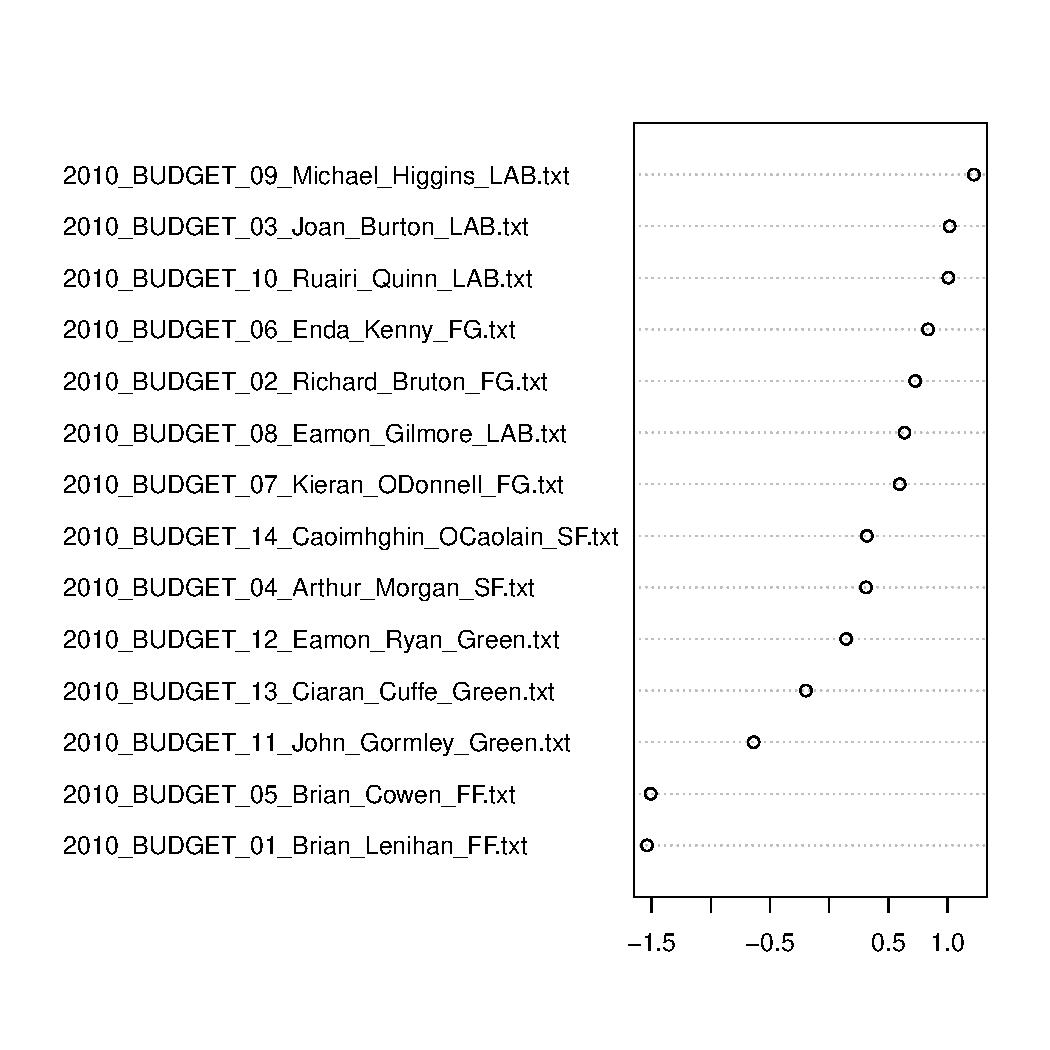
\includegraphics[width=\maxwidth]{figures/minimal-unnamed-chunk-6} 

}



\end{knitrout}


This plot indicates the position
of each of the documents. We can group documents by their attribute values when creating the word-frequency matrix: 

\begin{knitrout}
\definecolor{shadecolor}{rgb}{0.969, 0.969, 0.969}\color{fgcolor}\begin{kframe}
\begin{alltt}
\hlstd{partyMat} \hlkwb{<-} \hlkwd{dfm}\hlstd{(ieBudgets2010,} \hlkwc{group} \hlstd{=} \hlstr{"party"}\hlstd{)}
\end{alltt}
\begin{verbatim}
## Creating dfm: ... aggregating by group: party...complete ... done.
\end{verbatim}
\begin{alltt}
\hlstd{partyMat[,} \hlnum{1}\hlopt{:}\hlnum{5}\hlstd{]}
\end{alltt}
\begin{verbatim}
##        words
## docs      €  —   a abandoned abandoning
##   FF     35  5  78         0          0
##   FG     31  9 162         0          0
##   Green 108 23 326         2          1
##   LAB    75  9 288         0          0
##   SF     85  4 159         0          0
\end{verbatim}
\end{kframe}
\end{knitrout}


which allows us to scale according to a particular party or year, for example:

\begin{knitrout}
\definecolor{shadecolor}{rgb}{0.969, 0.969, 0.969}\color{fgcolor}\begin{kframe}
\begin{alltt}
\hlstd{partyModel} \hlkwb{<-} \hlkwd{ca}\hlstd{(}\hlkwd{t}\hlstd{(partyMat),} \hlkwc{nd} \hlstd{=} \hlnum{1}\hlstd{)}
\hlkwd{dotchart}\hlstd{(partyModel}\hlopt{$}\hlstd{colcoord[}\hlkwd{order}\hlstd{(partyModel}\hlopt{$}\hlstd{colcoord[,} \hlnum{1}\hlstd{]),} \hlnum{1}\hlstd{],} \hlkwc{labels} \hlstd{= partyModel}\hlopt{$}\hlstd{colnames[}\hlkwd{order}\hlstd{(partyModel}\hlopt{$}\hlstd{colcoord[,}
    \hlnum{1}\hlstd{])])}
\end{alltt}
\end{kframe}

{\centering 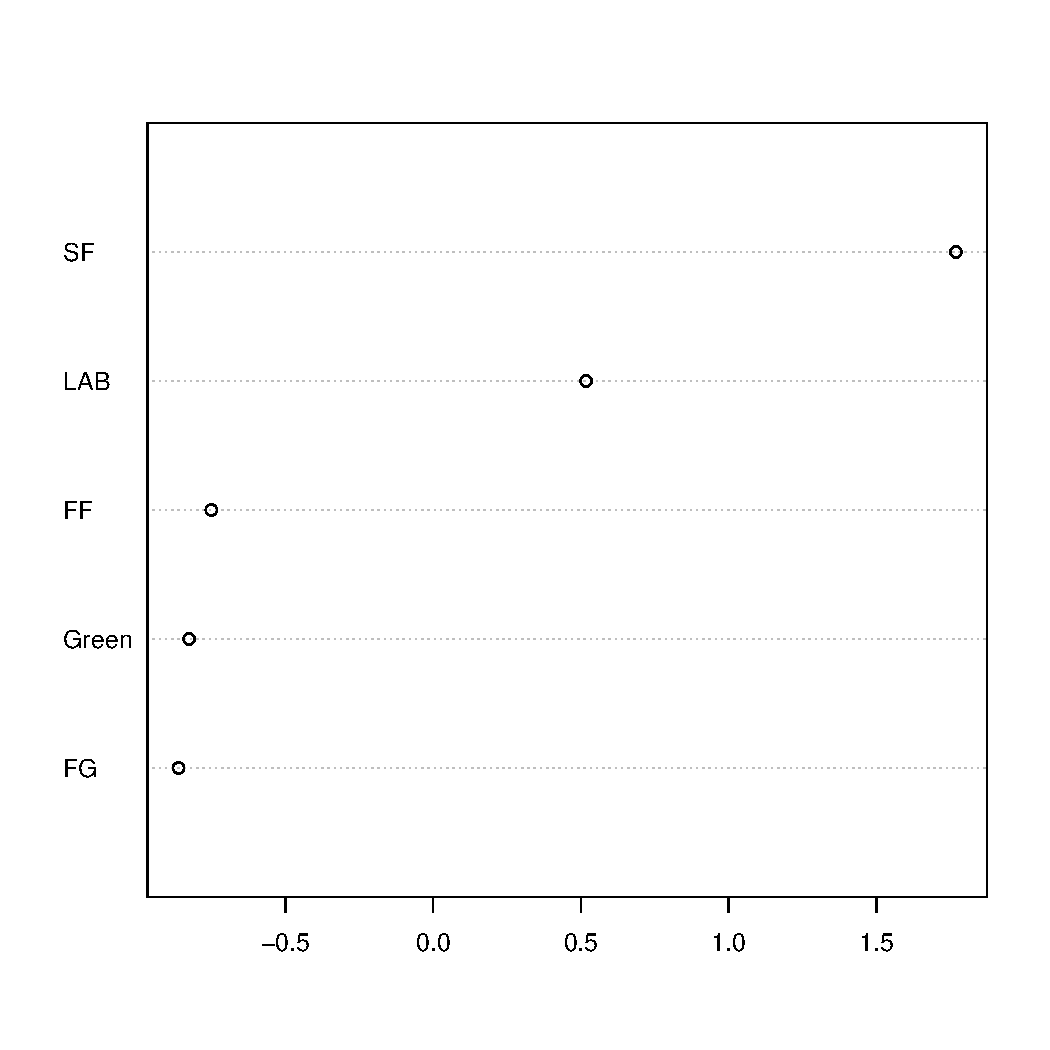
\includegraphics[width=\maxwidth]{figures/minimal-unnamed-chunk-8} 

}



\end{knitrout}


